\documentclass{article}
\usepackage{enumitem,graphicx,titling,units,braket,amsthm, amsmath,amssymb,mathtools,textcomp,tikz,pgfplots,listings,hyperref, physics, listings, color, float}

\newcommand\numberthis{\addtocounter{equation}{1}\tag{\theequation}}
\allowdisplaybreaks[1]

\makeatletter
\def\myitem{%
   \@ifnextchar[ \@myitem{\@noitemargtrue\@myitem[\@itemlabel]}}
\def\@myitem[#1]{\item[#1]\mbox{}\\\hspace*{\dimexpr-\labelwidth-\labelsep}}
\makeatother

\newtheorem{theorem}{Theorem}
\newtheorem{corollary}[theorem]{Corollary}
\newtheorem{conjecture}[theorem]{Conjecture}

\lstset{
	tabsize=4,
	rulecolor=,
	language=python,
        basicstyle=\scriptsize,
        upquote=true,
        aboveskip={1.5\baselineskip},
        columns=fixed,
        showstringspaces=false,
        extendedchars=true,
        breaklines=true,
        prebreak = \raisebox{0ex}[0ex][0ex]{\ensuremath{\hookleftarrow}},
        frame=single,
        showtabs=false,
        showspaces=false,
        showstringspaces=false,
        identifierstyle=\ttfamily,
        keywordstyle=\color[rgb]{0,0,1},
        commentstyle=\color[rgb]{0.133,0.545,0.133},
        stringstyle=\color[rgb]{0.627,0.126,0.941},
}

\begin{document}
	\setlength{\droptitle}{-10em}
	\title{Homework 4}
	\author{Andrew Lei\\Arizona State University}
	\maketitle
	
	\begin{enumerate}
		\item I picked the keyword Harambe.
		\item I tried Latent Dirichlet with 5, 10, and 20 topics. Five topics seemed to not provide as much of a range as I would have liked, whereas ten had some duplicates (e.g., topics about Halloween/costumes), and twenty with even more. Here are the topics (see `10topics.csv'):
		\begin{enumerate}[label=(\roman*)]
			\item 0.097*"haramb" + 0.038*"meme" + 0.035*"good" + 0.032*"basic"
			\item 0.182*"haramb" + 0.104*"like" + 0.093*"squad" + 0.061*"wshhcomedi"
			\item 0.129*"haramb" + 0.025*"kill" + [two inappropriate words excluded]
			\item 0.120*"haramb" + 0.023*"just" + 0.015*"gorilla" + 0.014*"night"
			\item 0.098*"haramb" + 0.076*"halloween" + 0.047*"dress" + 0.041*"parti"
			\item 0.164*"000" + 0.111*"haramb" + 0.094*"make" + 0.087*"ll"
			\item 0.106*"haramb" + 0.031*"rip" + 0.030*"now" + 0.018*"dead"
			\item 0.097*"haramb" + 0.023*"like" + 0.022*"don" + 0.016*"will"
			\item 0.120*"haramb" + 0.046*"sexi" + 0.045*"costum" + 0.039*"consult"
			\item 0.103*"haramb" + 0.078*"blacklivesmatt" + 0.077*"dio" + 0.077*"fratelloscimmia"
		\end{enumerate}
		Here are my interpretations of the topics provided by LDA:
		\begin{enumerate}[label=(\roman*)]
			\item Harambe as a meme
			\item Unclear
			\item Harambe's death / mourning Harambe
			\item Possibly `Harambe was just a gorilla'
			\item Harambe Halloween costumes
			\item Unclear
			\item Mourning Harambe
			\item Unclear
			\item Harambe Halloween costumes
			\item Unclear; something involving Harambe and Black Lives Matter, but I don't see the connection.
		\end{enumerate}
		
		I saved the topics and the topic each tweet was assigned to in separate files.
		
		\item All of the topics seemed to be mostly negative. However, the first topic did have some positive sentiment:
		\begin{figure}[H]
			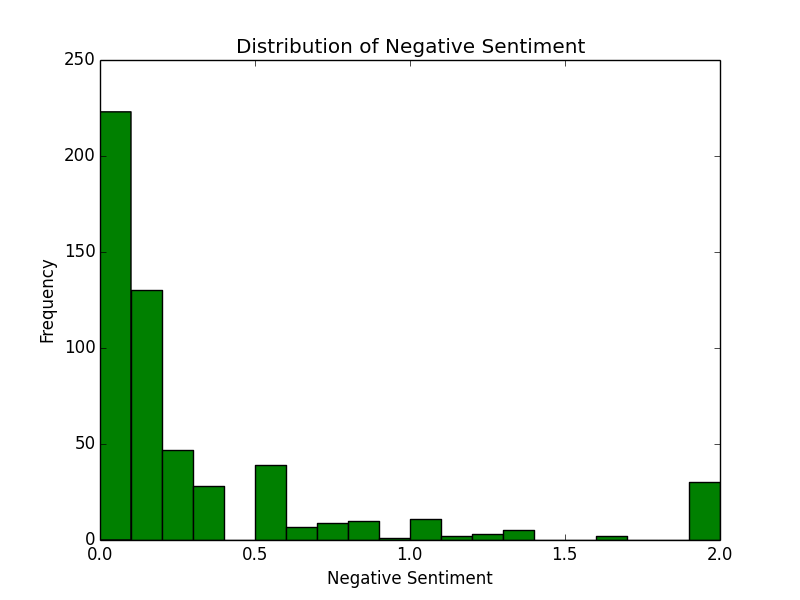
\includegraphics[scale=0.35]{0neg.png}
			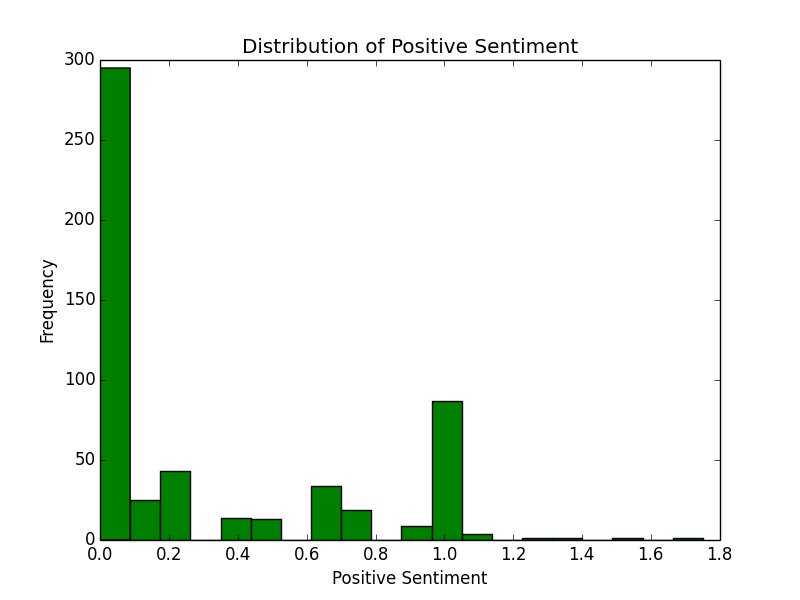
\includegraphics[scale=0.35]{0pos.png}
			\begin{center}
			\caption{Negative and positive sentiment distributions for first topic}
			\end{center}
		\end{figure}
		As you can see, most of the non-neutral sentiment is negative, but most of that negative sentiment is mild, with the exception of a bit of harshly negative sentiment. On the other hand, there is a good deal of somewhat-enthusiastic positive sentiment for this topic. Perhaps some are tired or annoyed of the meme, while others are still enthusiastic about it.\\
		The third topic I believe related to Harambe's death, so it's unsurprising that it appears to be somewhat negative.
		\begin{figure}[H]
			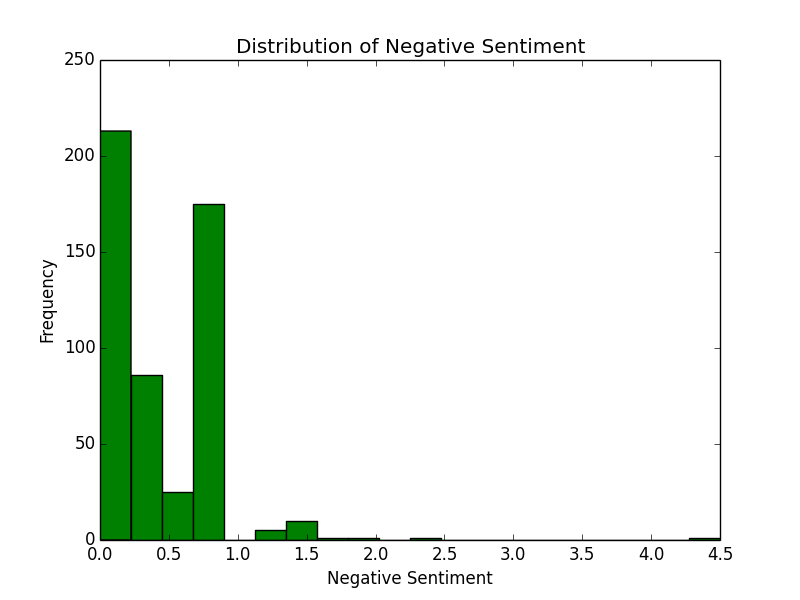
\includegraphics[scale=0.35]{2neg.png}
			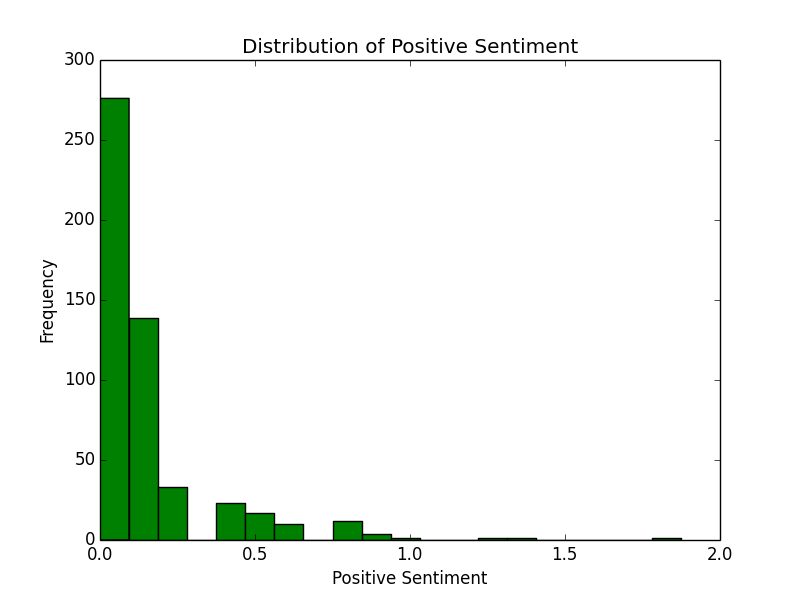
\includegraphics[scale=0.35]{2pos.png}
			\begin{center}
			\caption{Negative and positive sentiment distributions for third topic}
			\end{center}
		\end{figure}		
		
		Topic five I believe related to Harambe Halloween costumes. It seems Twitter quite overwhelmingly disapproves, but, strangely enough, the ninth topic, which also seems to relate to Harambe Halloween costumes, seems to be much more neutral (albeit still somewhat negative). It is, perhaps, a slightly different topic, though; the word `sexy' is part of the topic, so I believe the ninth topic refers more to Harambe costumes worn by women (or costumes worn by women).
		\begin{figure}[H]
			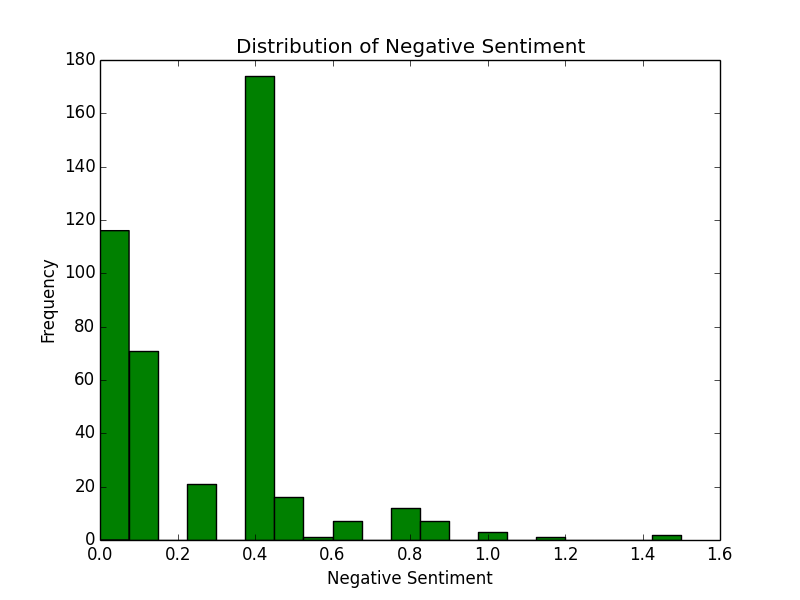
\includegraphics[scale=0.35]{4neg.png}
			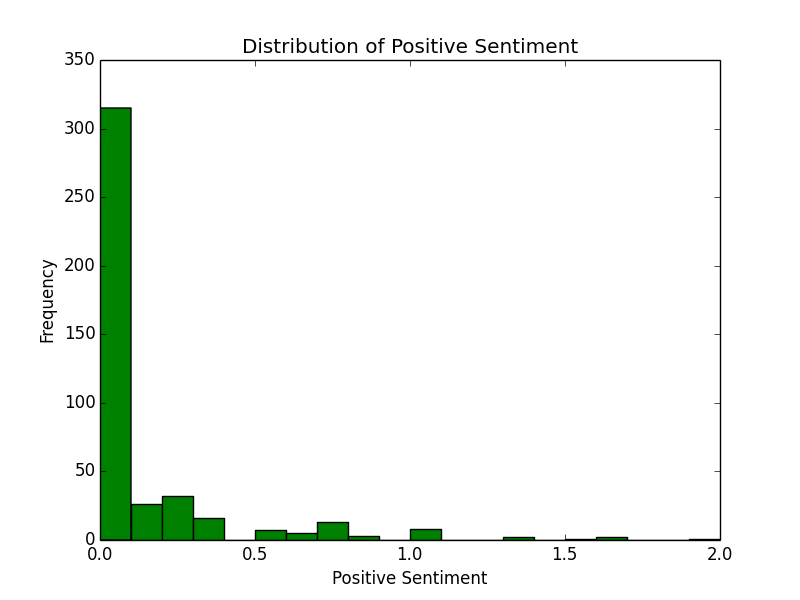
\includegraphics[scale=0.35]{4pos.png}
			\begin{center}
			\caption{Negative and positive sentiment distributions for fifth topic}
			\end{center}
		\end{figure}
		
		Topic ten, having something to do with Black Lives Matter apparently, is almost completely neutral.
		
		\begin{figure}[H]
			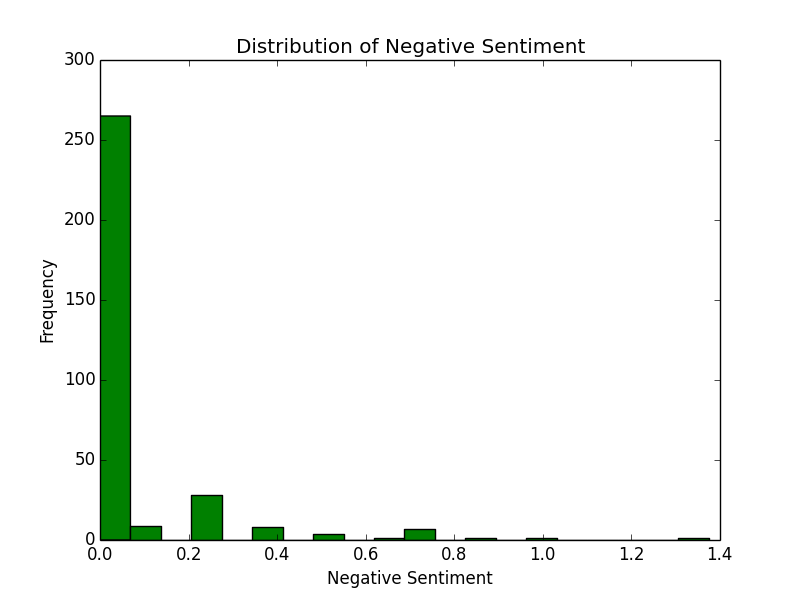
\includegraphics[scale=0.35]{9neg.png}
			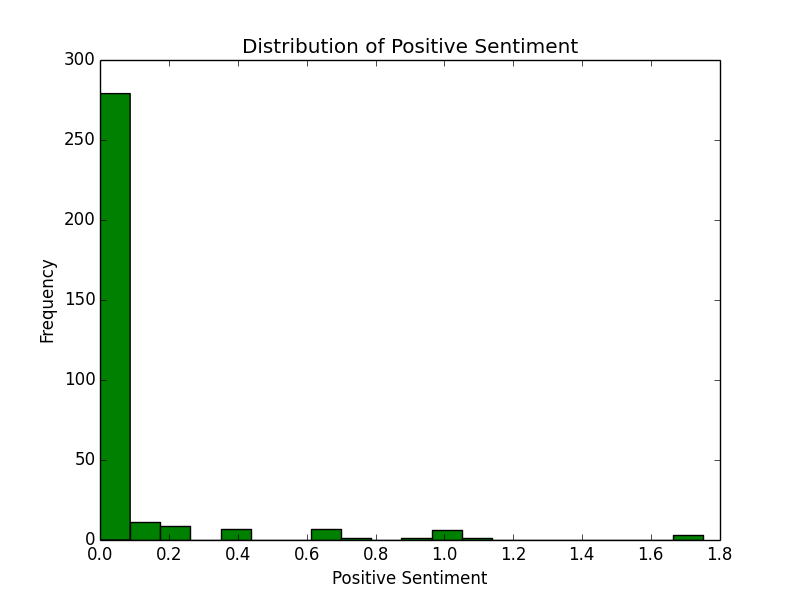
\includegraphics[scale=0.35]{9pos.png}
			\begin{center}
			\caption{Negative and positive sentiment distributions for tenth topic}
			\end{center}
		\end{figure}
		
		\begin{figure}[H]
			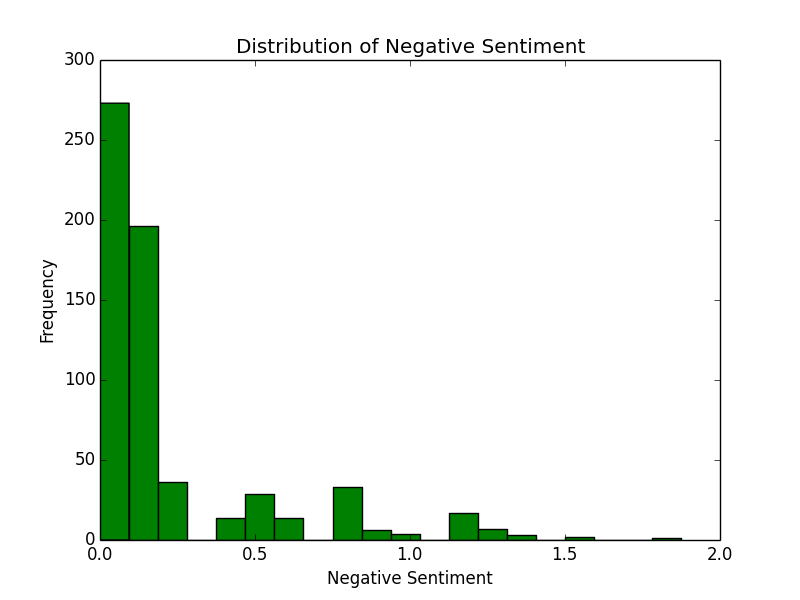
\includegraphics[scale=0.35]{8neg.png}
			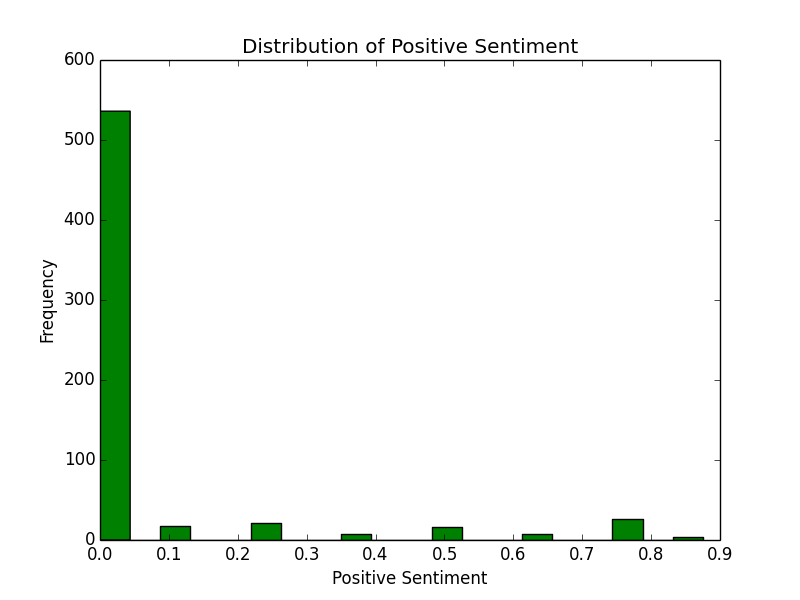
\includegraphics[scale=0.35]{8pos.png}
			\begin{center}
			\caption{Negative and positive sentiment distributions for ninth topic}
			\end{center}
		\end{figure}
		Topics two and six seem to have quite a bit of negative sentiment, but I was not able to interpret the topic, so I'm not sure what they mean.
		\begin{figure}[H]
			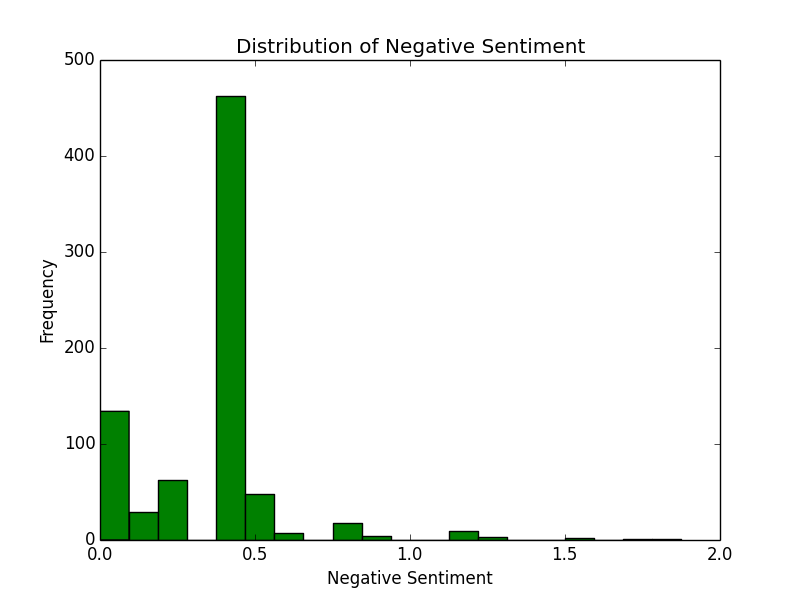
\includegraphics[scale=0.35]{1neg.png}
			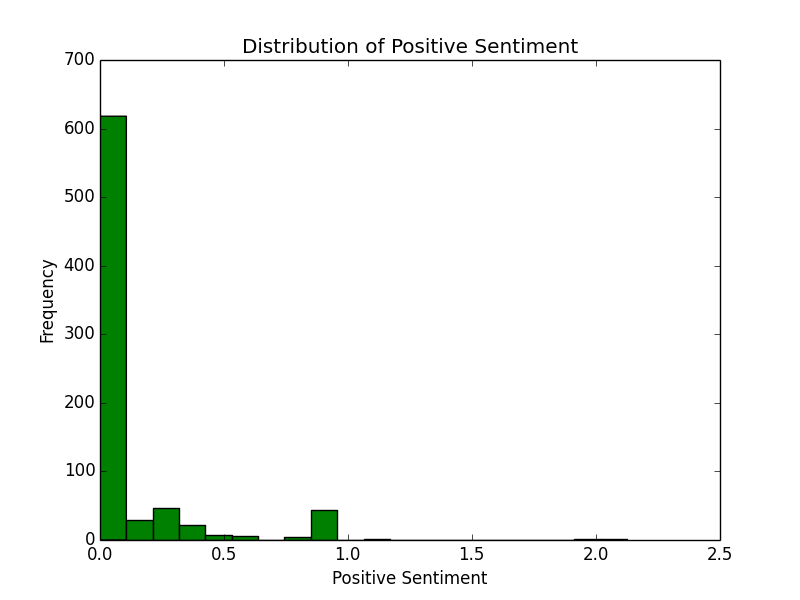
\includegraphics[scale=0.35]{1pos.png}
			\begin{center}
			\caption{Negative and positive sentiment distributions for second topic}
			\end{center}
		\end{figure}
		
		\begin{figure}[H]
			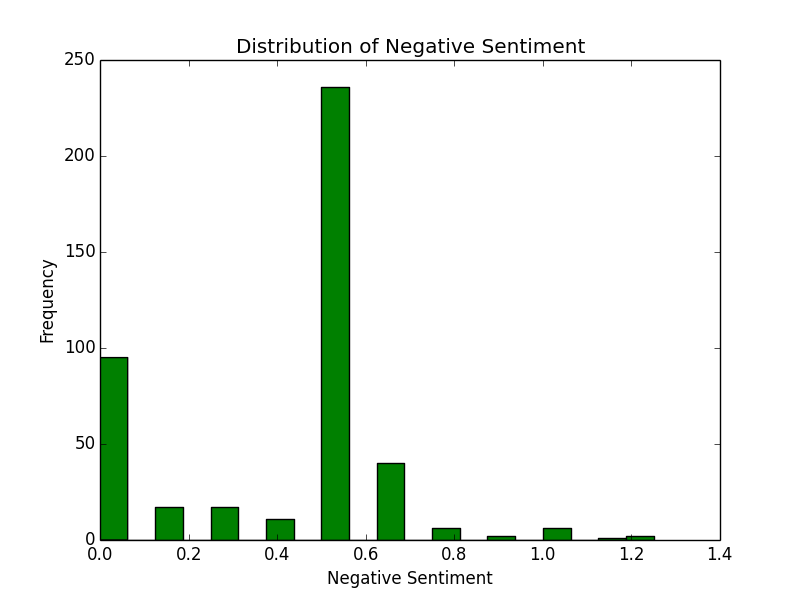
\includegraphics[scale=0.35]{5neg.png}
			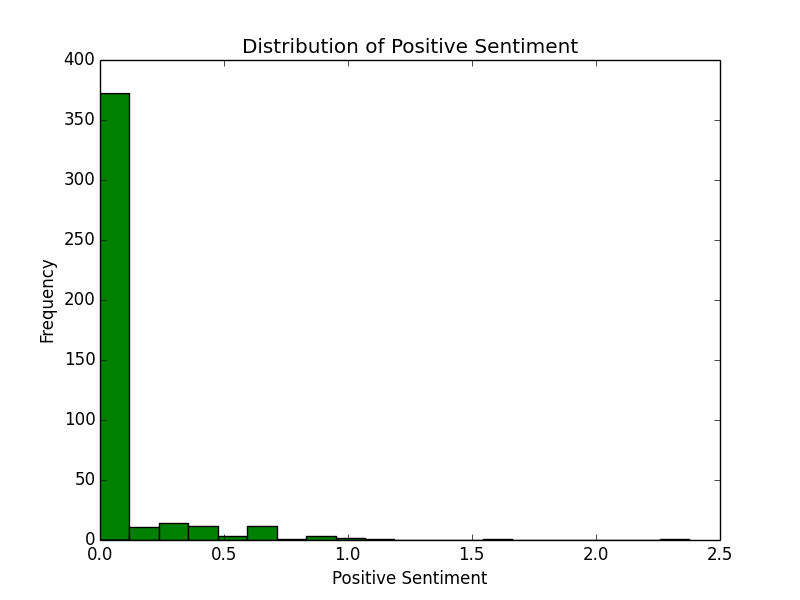
\includegraphics[scale=0.35]{5pos.png}
			\begin{center}
			\caption{Negative and positive sentiment distributions for sixth topic}
			\end{center}
		\end{figure}
		
		Finally, the rest of the topics (topics four, seven, and eight) just seem to be generally moderately negative without anything particularly noteworthy.
		\begin{figure}[H]
			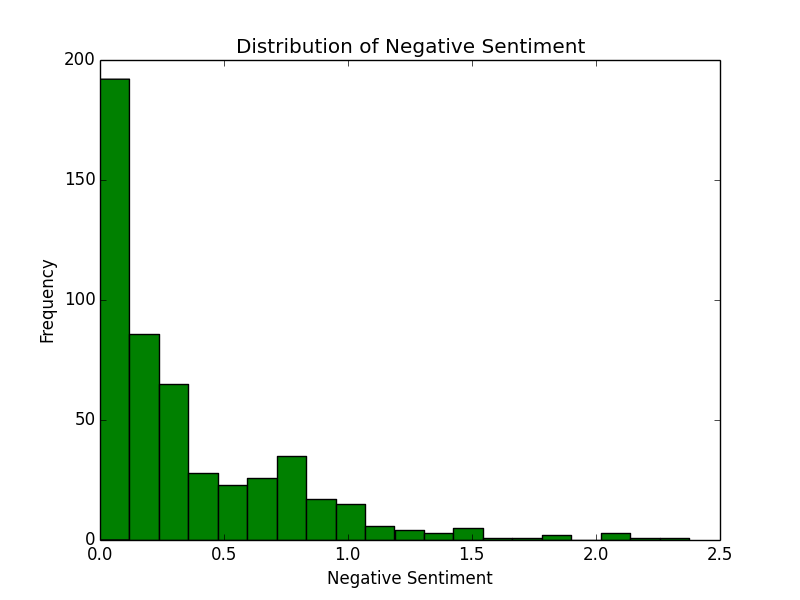
\includegraphics[scale=0.35]{3neg.png}
			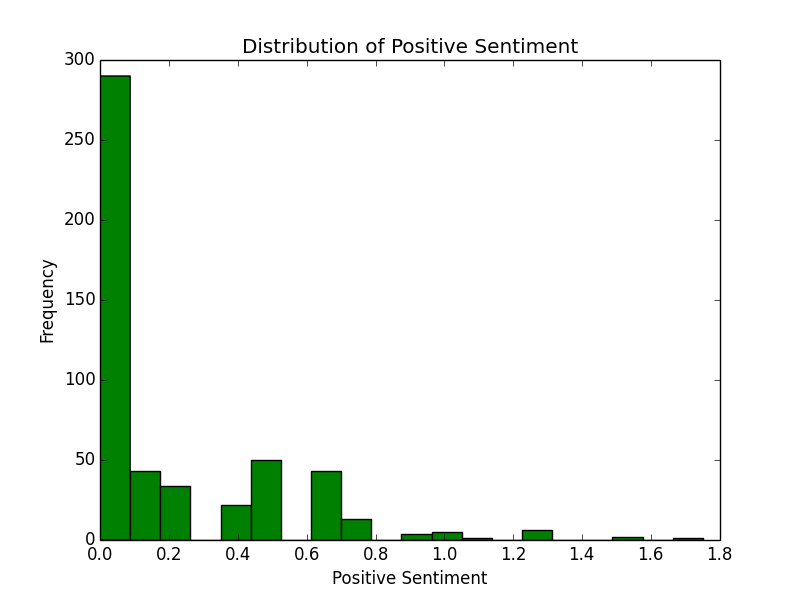
\includegraphics[scale=0.35]{3pos.png}
			\begin{center}
			\caption{Negative and positive sentiment distributions for fourth topic}
			\end{center}
		\end{figure}
		
		\begin{figure}[H]
			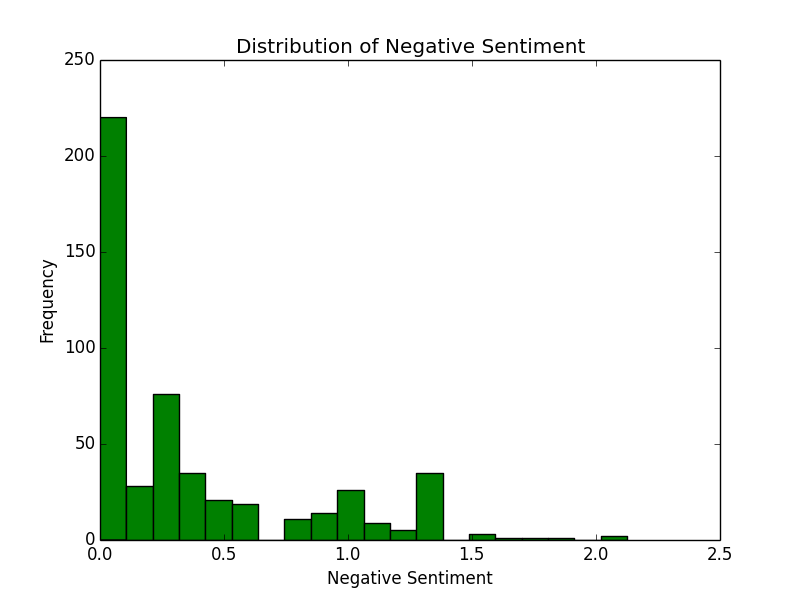
\includegraphics[scale=0.35]{6neg.png}
			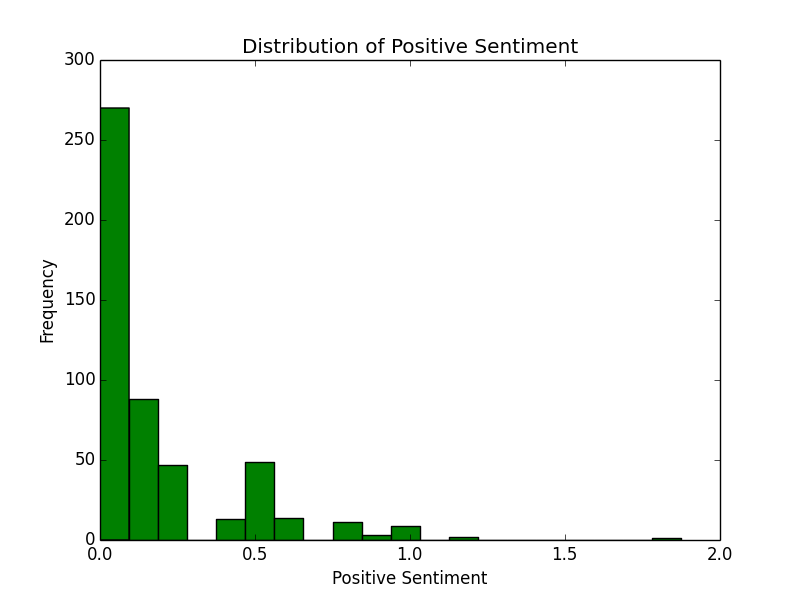
\includegraphics[scale=0.35]{6pos.png}
			\begin{center}
			\caption{Negative and positive sentiment distributions for seventh topic}
			\end{center}
		\end{figure}
		
		\begin{figure}[H]
			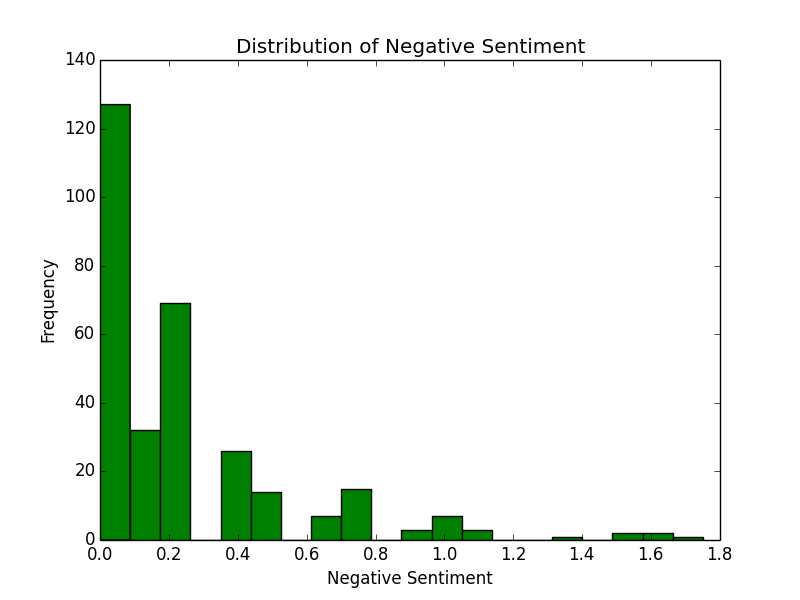
\includegraphics[scale=0.35]{7neg.png}
			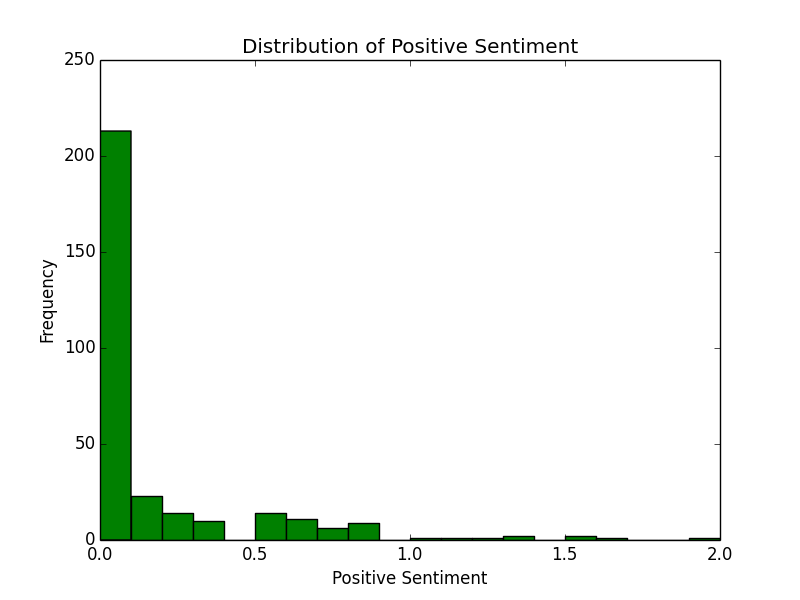
\includegraphics[scale=0.35]{7pos.png}
			\begin{center}
			\caption{Negative and positive sentiment distributions for eighth topic}
			\end{center}
		\end{figure}
		
	\end{enumerate}
	
\end{document}